\documentclass[journal]{IEEEtran}
\usepackage[a5paper, margin=10mm, onecolumn]{geometry}
\usepackage{tfrupee} 

\setlength{\headheight}{1cm}
\setlength{\headsep}{0mm} 

\usepackage{gvv-book}
\usepackage{gvv}
\usepackage{amsmath,amssymb,amsfonts,amsthm}
\usepackage{algorithmic}
\usepackage{graphicx}
\usepackage{textcomp}
\usepackage{xcolor}
\usepackage{txfonts}
\usepackage{listings}
\usepackage{enumitem}
\usepackage{mathtools}
\usepackage{gensymb}
\usepackage{comment}
\usepackage[breaklinks=true]{hyperref}
\usepackage{tkz-euclide} 
\usepackage{listings}
\def\inputGnumericTable{}                      
\usepackage[latin1]{inputenc}                                
\usepackage{color}                                         
\usepackage{array}                                            
\usepackage{longtable}                                       
\usepackage{calc}                                             
\usepackage{multirow}                                         
\usepackage{hhline}                                           
\usepackage{ifthen}                                           
\usepackage{lscape}
\usepackage{tikz}
\usetikzlibrary{patterns}
\begin{document}


\vspace{3cm}


\title{GATE 2024 - General Aptitude \& Ecology (EY)}
\author{ee25btech11034-Kishora Karthik}
\maketitle

{\let\newpage\relax\maketitle}

\renewcommand{\thefigure}{\theenumi}
\renewcommand{\thetable}{\theenumi}
\setlength{\intextsep}{10pt} 

\section*{\textbf{General Aptitude}}
\textbf{Q.1 to Q.5 carry one mark each.}
 
\begin{enumerate}
    \item If `$\rightarrow$' denotes increasing order of intensity, then the meaning of the words [simmer $\rightarrow$ seethe $\rightarrow$ smolder] is analogous to [break $\rightarrow$ raze $\rightarrow$ \underline{\hspace{3cm}} ]. Which one of the given options is appropriate to fill the blank?
    \begin{multicols}{2}
    \begin{enumerate}
        \item obfuscate
        \item obliterate
        \item fracture
        \item fissure
    \end{enumerate}
    \end{multicols}
\hfill{(GATE EY 2024)}

    \item In a locality, the houses are numbered in the following way: The house-numbers on one side of a road are consecutive odd integers starting from $301$, while the house-numbers on the other side of the road are consecutive even numbers starting from $302$. The total number of houses is the same on both sides of the road. If the difference of the sum of the house-numbers between the two sides of the road is $27$, then the number of houses on each side of the road is
    \begin{multicols}{2}
    \begin{enumerate}
        \item $27$
        \item $52$
        \item $54$
        \item $26$
    \end{enumerate}
    \end{multicols}
\hfill{(GATE EY 2024)}

    \item For $p \neq 1$, $q \neq 1$, $(\frac{p}{q})^{p-q} = (\frac{q}{p})^{q-p}$. Then
    \begin{multicols}{2}
    \begin{enumerate}
        \item $p+q = 0$
        \item $p-q = -1$
        \item $\sqrt{q} = \sqrt{p}$
        \item $\sqrt[p]{q} = \sqrt[q]{p}$
    \end{enumerate}
    \end{multicols}
\hfill{(GATE EY 2024)}

    \item Which one of the given options is a possible value of $x$ in the following sequence? $3, 7, 15, x, 63, 127, 255$
    \begin{multicols}{2}
    \begin{enumerate}
        \item $35$
        \item $40$
        \item $45$
        \item $31$
    \end{enumerate}
    \end{multicols}
\hfill{(GATE EY 2024)}

    \item On a given day, how many times will the second-hand and the minute-hand of a clock cross each other during the clock time 12:05:00 hours to 12:55:00 hours?
    \begin{multicols}{2}
    \begin{enumerate}
        \item $50$
        \item $49$
        \item $55$
        \item $1$
    \end{enumerate}
    \end{multicols}
\hfill{(GATE EY 2024)}

\textbf{Q.6 to Q.10 carry two marks each.}

\item In the given text, the blanks are numbered (i)-(iv). Select the best match for all the blanks. \\
From the ancient Athenian arena to the modern Olympic stadiums, athletics \underline{\hspace{0.5cm}(i)\hspace{0.5cm}} the potential for a spectacle. The crowd \underline{\hspace{0.5cm}(ii)\hspace{0.5cm}} with bated breath as the Olympian artist twists his body, stretching the javelin behind him. Twelve strides in, he begins to cross-step. Six cross-steps \underline{\hspace{0.5cm}(iii)\hspace{0.5cm}} in an abrupt stop on his left foot. As his body \underline{\hspace{0.5cm}(iv)\hspace{0.5cm}} like a door turning on a hinge, the javelin is launched skyward at a precise angle.
    \begin{enumerate}
        \item (i) hold (ii) waits (iii) culminates (iv) pivot
        \item (i) holds (ii) wait (iii) culminates (iv) pivot
        \item (i) holds (ii) waits (iii) culminate (iv) pivots
        \item (i) hold (ii) wait (iii) culminate (iv) pivots
    \end{enumerate}
\hfill{(GATE EY 2024)}

\item Three distinct sets of indistinguishable twins are to be seated at a circular table that has $8$ identical chairs. Unique seating arrangements are defined by the relative positions of the people. How many unique seating arrangements are possible such that each person is sitting next to their twin?
    \begin{multicols}{2}
    \begin{enumerate}
        \item $12$
        \item $14$
        \item $10$
        \item $28$
    \end{enumerate}
    \end{multicols}
\hfill{(GATE EY 2024)}

\item The chart given below compares the Installed Capacity (MW) of four power generation technologies, T1, T2, T3, and T4, and their Electricity Generation (MWh) in a time of $1000$ hours (h).
\begin{figure}[!ht]
    \centering
    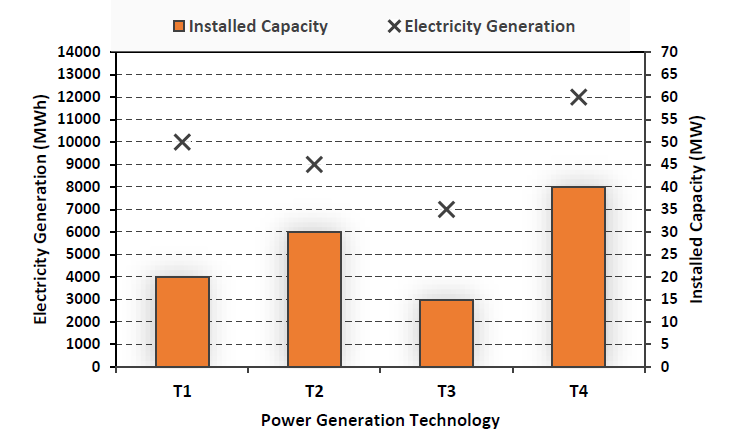
\includegraphics[width=0.3\columnwidth]{figs/Q-8.png}
    \caption{Question 8: Comparison of Installed Capacity and Electricity Generation for four power technologies.}
    \label{Q.8}
\end{figure}
The Capacity Factor of a power generation technology is:
$$ \text{Capacity Factor} = \frac{\text{Electricity Generation (MWh)}}{\text{Installed Capacity (MW)} \times 1000 \text{(h)}} $$
Which one of the given technologies has the highest Capacity Factor?
    \begin{multicols}{2}
    \begin{enumerate}
        \item T1
        \item T2
        \item T3
        \item T4
    \end{enumerate}
    \end{multicols}
\hfill{(GATE EY 2024)}

\item In the $4 \times 4$ array shown below, each cell of the first three columns has either a cross (X) or a number, as per the given rule.
\begin{figure}[!ht]
    \centering
    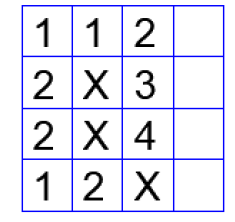
\includegraphics[width=0.4\columnwidth]{figs/Q-9.png}
    \caption{Question 9: A 4x4 array with crosses and numbers in the first three columns.}
    \label{Q.9}
\end{figure}
Rule: The number in a cell represents the count of crosses around its immediate neighboring cells (left, right, top, bottom, diagonals). As per this rule, the maximum number of crosses possible in the empty column is
    \begin{multicols}{2}
    \begin{enumerate}
        \item $0$
        \item $1$
        \item $2$
        \item $3$
    \end{enumerate}
    \end{multicols}
\hfill{(GATE EY 2024)}

\item During a half-moon phase, the Earth-Moon-Sun form a right triangle. If the Moon-Earth-Sun angle at this half-moon phase is measured to be $89.85^{\degree}$, the ratio of the Earth-Sun and Earth-Moon distances is closest to
    \begin{multicols}{2}
    \begin{enumerate}
        \item $328$
        \item $382$
        \item $238$
        \item $283$
    \end{enumerate}
    \end{multicols}
\hfill{(GATE EY 2024)}
\end{enumerate}
\bigskip
\centering {\textbf{\large{END OF GENERAL APTITUDE}}}
\clearpage

\section*{\textbf{Ecology and Evolution (EY)}}
\textbf{Q.11 to Q.35 carry one mark each.}
\begin{enumerate}
\setcounter{enumi}{10}

\item The molecular clock model assumes that mutation rates are
    \begin{multicols}{2}
    \begin{enumerate}
        \item equal for all genes.
        \item constant for a gene.
        \item variable across geographical regions.
        \item variable across geological time.
    \end{enumerate}
    \end{multicols}
\hfill{(GATE EY 2024)}

\item The intermediate disturbance hypothesis states that species diversity is highest at intermediate levels of disturbance. This is because
    \begin{enumerate}
        \item common species are not affected by disturbance.
        \item a few species are able to survive in high disturbance.
        \item there is competitive exclusion in low disturbance.
        \item rare species are able to survive in high disturbance.
    \end{enumerate}
\hfill{(GATE EY 2024)}

\item A few years ago, a very small population of zebrafish became isolated by a newly built dam. As a result, which statement is most likely to be true about this population of zebrafish now?
    \begin{enumerate}
        \item Genetic variability is low.
        \item Fixation of genotypes due to drift is low.
        \item Inbreeding is low.
        \item Mutation rate is high.
    \end{enumerate}
\hfill{(GATE EY 2024)}

\item A researcher measures the tree heights of all individuals of a species in a forest. Which one of the following is NOT a measure of variability in the sample?
    \begin{multicols}{2}
    \begin{enumerate}
        \item Standard deviation
        \item Standard error
        \item Median
        \item Variance
    \end{enumerate}
    \end{multicols}
\hfill{(GATE EY 2024)}

\item Individual lizards were repeatedly presented with a predator model. Over successive trials, they showed a reduction in the duration of their alarm response. Which one of the following is this an example of?
    \begin{multicols}{2}
    \begin{enumerate}
        \item Imitation
        \item Imprinting
        \item Habituation
        \item Sensitisation
    \end{enumerate}
    \end{multicols}
\hfill{(GATE EY 2024)}

\item Among the following vertebrate classes, biparental care is most common in
    \begin{multicols}{2}
    \begin{enumerate}
        \item amphibians.
        \item birds.
        \item fishes.
        \item mammals.
    \end{enumerate}
    \end{multicols}
\hfill{(GATE EY 2024)}

\item Based on paleontological evidence, eukaryotic organisms are estimated to have first evolved
    \begin{enumerate}
        \item more than $750$ million years ago.
        \item $750$ to $500$ million years ago.
        \item $500$ to $250$ million years ago.
        \item $65$ million years ago.
    \end{enumerate}
\hfill{(GATE EY 2024)}

\item In a population, there are two morphs, $A$ and $B$, which reproduce at equal rates. $A$ mutates to $B$ with probability $p_1$, and $B$ mutates to $A$ with probability $p_2$ such that $p_1 \gg p_2$ (that is, $p_1$ is much greater than $p_2$). Over time, which one of the following statements would be true about this population?
    \begin{enumerate}
        \item Both morphs $A$ and $B$ will become equally abundant.
        \item Morph $A$ will dominate the population.
        \item Morph $B$ will dominate the population.
        \item Both morphs $A$ and $B$ will go extinct.
    \end{enumerate}
\hfill{(GATE EY 2024)}

\item Terrestrial plants conduct gas exchange through stomata. Having only few stomata on the leaf surface is a common adaptation to which one of the following conditions?
    \begin{multicols}{2}
    \begin{enumerate}
        \item High aridity
        \item High pH
        \item Low UV radiation
        \item Low soil nitrogen
    \end{enumerate}
    \end{multicols}
\hfill{(GATE EY 2024)}

\item Which one of the following is a result of antagonistic coevolution?
    \begin{enumerate}
        \item Convergent evolution of bird wings and bat wings
        \item Adaptive radiation of beak shape in Darwin's finches
        \item Caterpillars that feed on chemically-defended host plants
        \item Specialised morphology of orchid flowers for pollination
    \end{enumerate}
\hfill{(GATE EY 2024)}

\item A classical metapopulation at equilibrium is made up of local populations with
    \begin{enumerate}
        \item no dispersal between them.
        \item no local colonisation or extinction.
        \item weak dispersal between them.
        \item panmictically breeding individuals across populations.
    \end{enumerate}
\hfill{(GATE EY 2024)}

\item Which one of the following theories is supported by the distribution patterns of extinct flora such as Glossopteris across South America, Africa and Australia, and extant marsupial mammals across South America and Australia?
    \begin{enumerate}
        \item Darwin's theory of natural selection
        \item Wegener's theory of continental drift
        \item Levins' theory of metapopulations
        \item MacArthur and Wilson's theory of island biogeography
    \end{enumerate}
\hfill{(GATE EY 2024)}

\item In linear regression, mean squared regression (effect variance) divided by mean squared error (error variance) is called the
    \begin{multicols}{2}
    \begin{enumerate}
        \item p-value.
        \item F-statistic.
        \item t-statistic.
        \item R-squared value.
    \end{enumerate}
    \end{multicols}
\hfill{(GATE EY 2024)}

\item The figure shows the time-series of atmospheric CO2 concentration on Earth (graph not-to-scale). Which one of the factors given is the primary reason for the sudden increase in atmospheric CO2 concentration after $1950$?
\begin{figure}[!ht]
    \centering
    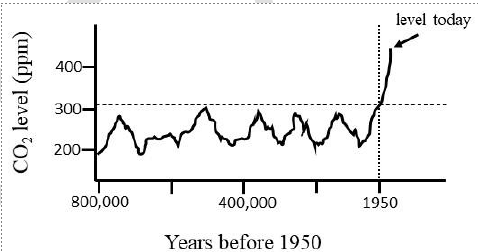
\includegraphics[width=0.3\columnwidth]{figs/Q-24.png}
    \caption{Question 24: Time-series of atmospheric CO2 concentration over the last 800,000 years.}
    \label{Q.24}
\end{figure}
    \begin{enumerate}
        \item Overfishing
        \item An increase in Arctic sea ice melting
        \item An increase in fossil fuel burning
        \item Volcanic eruptions
    \end{enumerate}
\hfill{(GATE EY 2024)}

\item The population size at which net recruitment is the highest is also when the greatest amount can be harvested, while ensuring the long-term survival of the population. The amount harvested at this population size is known as
    \begin{multicols}{2}
    \begin{enumerate}
        \item carrying capacity.
        \item maximum sustainable yield.
        \item maximum survival density.
        \item optimal recruitment.
    \end{enumerate}
    \end{multicols}
\hfill{(GATE EY 2024)}

\item The variance in male mating success is $V_m$ and that of females is $V_f$. Assuming that the sex ratio is $1:1$, in which one of the following mating systems is $V_m/V_f$ expected to be the greatest?
    \begin{multicols}{2}
    \begin{enumerate}
        \item Monogamy
        \item Random mating
        \item Polyandry
        \item Polygyny
    \end{enumerate}
    \end{multicols}
\hfill{(GATE EY 2024)}

\item Some air-breathing marine vertebrates such as whales, seals and marine turtles possess adaptations for long, deep dives. Which one or more of the following is/are examples of such adaptations?
    \begin{multicols}{2}
    \begin{enumerate}
        \item Tolerance to hypoxia
        \item Slow heart rate
        \item High levels of haemoglobin
        \item Salt tolerance
    \end{enumerate}
    \end{multicols}
\hfill{(GATE EY 2024)}

\item Which one or more of the following statements about evolution is/are true?
    \begin{enumerate}
        \item Evolution is change that is heritable across generations.
        \item Evolution occurs at the level of populations, not species.
        \item Evolution is a change in gene frequencies through time.
        \item Evolution occurs through natural selection, but not sexual selection.
    \end{enumerate}
\hfill{(GATE EY 2024)}

\item Which one or more of the following mammal species is/are endemic to India?
    \begin{multicols}{2}
    \begin{enumerate}
        \item One-horned rhinoceros
        \item Lion-tailed macaque
        \item Bengal tiger
        \item Cheetah
    \end{enumerate}
    \end{multicols}
\hfill{(GATE EY 2024)}

\item Under which one or more of the following conditions can altruism evolve in animal societies?
    \begin{enumerate}
        \item Individuals in a group are closely related to each other.
        \item Individuals live in a high resource, low risk environment.
        \item Individuals in a group mutually help each other at different times.
        \item Mating opportunities are equally distributed among individuals.
    \end{enumerate}
\hfill{(GATE EY 2024)}

\item Two species of fruit bats (Species $1$ and Species $2$) eat fruits of varying sizes. The curves shown represent the ecological niche for these two species. If the curves for both species were to completely overlap, which one or more of the statements given would be correct?
\begin{figure}[!ht]
    \centering
    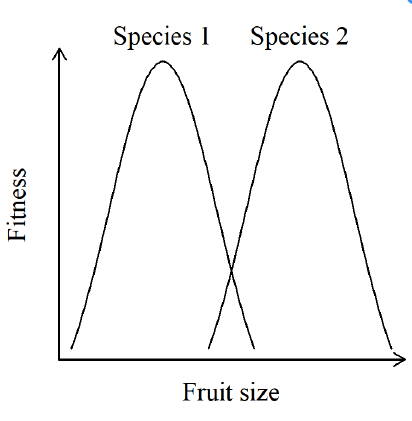
\includegraphics[width=0.6\columnwidth]{figs/Q-31.png}
    \caption{Question 31: Ecological niches of two fruit bat species based on fruit size and fitness.}
    \label{Q.31}
\end{figure}
    \begin{enumerate}
        \item There will be no resource competition between Species $1$ and Species $2$.
        \item One of the species may become extinct due to competitive exclusion.
        \item There will be little competition between Species $1$ and Species $2$.
        \item The two species will use identical resources.
    \end{enumerate}
\hfill{(GATE EY 2024)}

\item During the process of succession in a community, species that are good colonisers are gradually replaced by species that are good competitors. Which one or more of the following statements is/are consistent with this pattern?
    \begin{enumerate}
        \item Initially, there is great resource limitation.
        \item Keystone species must establish first to facilitate the later establishment of higher trophic level species.
        \item Trees are the climax stage of terrestrial communities and generally have low competitive ability, but high dispersal ability.
        \item For many taxa, there is a tradeoff between dispersal ability and local competitive ability.
    \end{enumerate}
\hfill{(GATE EY 2024)}

\item An ornamental shrub species was brought from Japan in the early $1800$s to India, where it was planted frequently in gardens and parks. The species persisted for many decades without spreading, and then began to spread invasively fifty years ago. Which one or more of the following processes could have led to it becoming invasive?
    \begin{enumerate}
        \item Evolutionary adaptation to the environment
        \item Open niches due to recent habitat degradation
        \item Climate change
        \item Recent introduction of a specialized herbivore of this shrub species
    \end{enumerate}
\hfill{(GATE EY 2024)}

\item Male voles pair with either a single female (monogamous) or with two females (polygynous) during a given breeding season. The probability of a male being polygynous in a breeding season is $0.2$. The reproductive success (number of offspring) of monogamous males is $2$, and of polygynous males is $3$. A male's expected reproductive success in a breeding season is \underline{\hspace{3cm}}. (Round off to one decimal place)
\hfill{(GATE EY 2024)}

\item Consider a randomly breeding population of squirrels with two morphs -- white striped and brown striped. In a population, $16\%$ are white striped individuals, while the rest are all brown striped. The trait for stripes is governed by one gene where the allele for brown stripes is dominant. Assuming Hardy-Weinberg equilibrium, the frequency of the allele for white stripes would be \underline{\hspace{3cm}}. (Round off to two decimal places)
\hfill{(GATE EY 2024)}

\textbf{Q.36 to Q.65 carry two marks each.}

\item Observations of algal species showed that their diversity was higher in pools where there were grazing snails compared to pools without snails. Which one of the following statements best explains this result?
    \begin{enumerate}
        \item Snails feed preferentially on the more abundant algal species.
        \item Snails avoid feeding on algal species.
        \item Snails feed only on the less abundant algal species.
        \item Snails feed equally on all the algal species irrespective of algal abundance.
    \end{enumerate}
\hfill{(GATE EY 2024)}

\item Which two of the following processes can result in a decline in heterozygosity in populations? \\
I) inbreeding; II) genetic drift; III) mutation; IV) random mating
    \begin{multicols}{2}
    \begin{enumerate}
        \item I and II
        \item II and III
        \item I and III
        \item II and IV
    \end{enumerate}
    \end{multicols}
\hfill{(GATE EY 2024)}

\item Given below is a table with ecological observations and processes. 
\begin{tabular}{|l|l|}
\hline
\textbf{Ecological observations} & \textbf{Processes} \\
\hline
P) Bright spotted pigmentation in & I) Kin selection \\
guppy males in low predation habitats & \\
\hline
Q) Vampire bats share blood meals & II) Sexual selection \\
\hline
R) Cooperative breeding in African & III) Reciprocal altruism \\
weaver birds & \\
\hline
\end{tabular} \\
Select the option that best matches each ecological observation with its corresponding process.
    \begin{multicols}{2}
    \begin{enumerate}
        \item P-III, Q-I, R-II
        \item P-II, Q-III, R-I
        \item P-I, Q-III, R-II
        \item P-II, Q-I, R-III
    \end{enumerate}
    \end{multicols}
\hfill{(GATE EY 2024)}

\item An ecologist must determine whether (i) the means of two independent samples differ, and (ii) there is an association between two continuous variables. Assuming that all samples are normally distributed, which one of the following options represents the most appropriate statistical tests for (i) and (ii), respectively?
    \begin{enumerate}
        \item (i) Spearman's correlation; (ii) Shapiro-Wilk test
        \item (i) Wilcoxon's matched pairs signed rank test; (ii) chi-squared test
        \item (i) t-test; (ii) Pearson's correlation
        \item (i) Kendall's test of concordance; (ii) Kolmogorov-Smirnov test
    \end{enumerate}
\hfill{(GATE EY 2024)}

\item Males of the swordtail fish \textit{Xiphophorus helleri} possess long tails, while those of \textit{X. maculatus} do not. Females of \textit{X. helleri} prefer males with longer tails. Interestingly, experimental studies show that females of \textit{X. maculatus} prefer \textit{X. maculatus} males with attached artificial long tails over those without. If the long-tailed \textit{Xiphophorus} species evolved from ancestors that lacked a long tail, which one of the following processes best explains the evolution of the observed preference among \textit{X. maculatus} females?
    \begin{multicols}{2}
    \begin{enumerate}
        \item Kin selection
        \item Sensory bias
        \item Group selection
        \item Runaway selection
    \end{enumerate}
    \end{multicols}
\hfill{(GATE EY 2024)}

\item Which one of the options given best matches vector to disease? \\
\begin{tabular}{ll}
\textbf{Vector} & \textbf{Disease} \\
I. Fleas & P. Kyasanur Forest Disease \\
II. Ticks & Q. Dengue \\
III. Mosquitoes & R. Plague \\
\end{tabular}
    \begin{multicols}{2}
    \begin{enumerate}
        \item I-R; II-P; III-Q
        \item I-P; II-R; III-Q
        \item I-R; II-Q; III-P
        \item I-P; II-Q; III-R
    \end{enumerate}
    \end{multicols}
\hfill{(GATE EY 2024)}

\item Optimal foraging theory predicts whether a foraging animal will be risk-prone, risk-averse or risk-insensitive depending on a utility function that describes the value of each additional food item to the animal. Risk-prone foraging is expected when the utility increases disproportionately with each additional food item encountered. Which one of the graphs shown depicts a scenario where risk-prone foraging would be expected?
\begin{figure}[!ht]
    \centering
    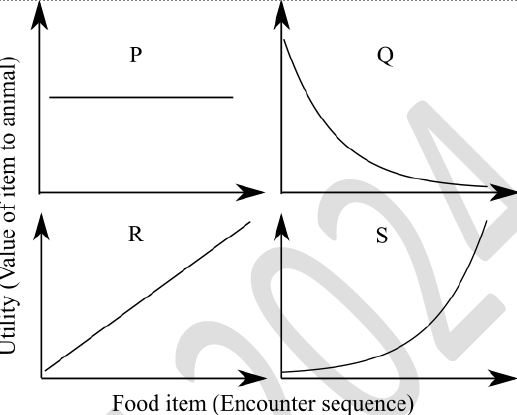
\includegraphics[width=0.3\columnwidth]{figs/Q-42.png}
    \caption{Question 42: Four graphs (P, Q, R, S) showing different utility functions for foraging.}
    \label{Q.42}
\end{figure}
    \begin{multicols}{4}
    \begin{enumerate}
        \item P
        \item Q
        \item R
        \item S
    \end{enumerate}
    \end{multicols}
\hfill{(GATE EY 2024)}

\item There are two species, $X$ and $Y$, with abundances $x$ and $y$, respectively. Species $X$ has growth rate $\alpha$, and species $Y$ has growth rate $\beta$. Assume that the sum of the species abundances is constant over time, i.e., $x + y = 1$. Let $x$ and $y$ follow the rate equations:
$$ \frac{dx}{dt} = \alpha x - \phi x, $$
$$ \frac{dy}{dt} = \beta y - \phi y, $$
where $\phi$ is the average species fitness. Which one of the following options correctly represents the expression for $\phi$?
    \begin{multicols}{2}
    \begin{enumerate}
        \item $\alpha x^2 + \beta y^2$
        \item $\alpha x + \beta y$
        \item $\frac{\alpha x + \beta y}{x^2 + y^2}$
        \item $\frac{1}{\alpha x + \beta y}$
    \end{enumerate}
    \end{multicols}
\hfill{(GATE EY 2024)}

\item The graphs shown represent the relationship between population size ($N$) and population growth rate ($\frac{dN}{dt}$). Which one of the following growth curves represents a density-dependent population that experiences a strong Allee effect?
\begin{figure}[!ht]
    \centering
    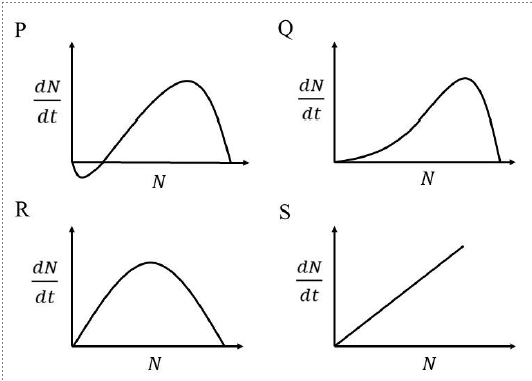
\includegraphics[width=0.3\columnwidth]{figs/Q-44.png}
    \caption{Question 44: Four graphs (P, Q, R, S) showing the relationship between population size (N) and population growth rate (dN/dt).}
    \label{Q.44}
\end{figure}
    \begin{multicols}{4}
    \begin{enumerate}
        \item P
        \item Q
        \item R
        \item S
    \end{enumerate}
    \end{multicols}
\hfill{(GATE EY 2024)}

\item The abundance ($X$) of a plant species with respect to the anthropogenic stressor habitat destruction ($h$) is shown. The solid and the dashed curves represent stable and unstable population equilibrium abundances, respectively. In the absence of any stochasticity, and with increasing values of $h$, what is the value of $h$ at which a sudden population collapse would occur?
\begin{figure}[!ht]
    \centering
    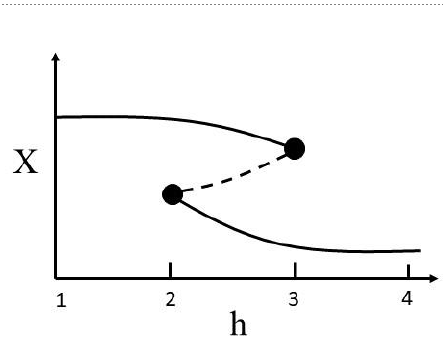
\includegraphics[width=0.3\columnwidth]{figs/Q-45.png}
    \caption{Question 45: Relationship between plant species abundance (X) and habitat destruction (h), showing stable and unstable equilibria.}
    \label{Q.45}
\end{figure}
    \begin{multicols}{4}
    \begin{enumerate}
        \item $2.5$
        \item $2$
        \item $4$
        \item $3$
    \end{enumerate}
    \end{multicols}
\hfill{(GATE EY 2024)}

\item Consider the graph shown, where $S$ is species richness and $A$ is area. $S$ and $A$ are log-transformed and the slope is not equal to $1$. The relationship between untransformed $S$ and $A$ follows a/an
\begin{figure}[!ht]
    \centering
    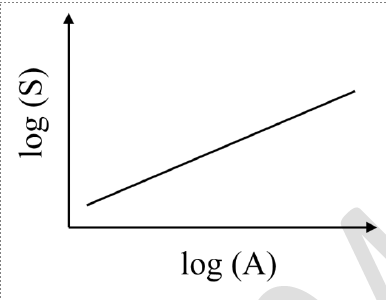
\includegraphics[width=0.3\columnwidth]{figs/Q-46.png}
    \caption{Question 46: Log-log plot of species richness (S) versus area (A).}
    \label{Q.46}
\end{figure}
    \begin{enumerate}
        \item linear relationship.
        \item power law.
        \item exponential relationship.
        \item Michaelis-Menten function.
    \end{enumerate}
\hfill{(GATE EY 2024)}

\item The graph shows the rank-abundance relationships for species in three communities, P, Q and R. Which one of the following statements is true with respect to the evenness of the three communities?
\begin{figure}[!ht]
    \centering
    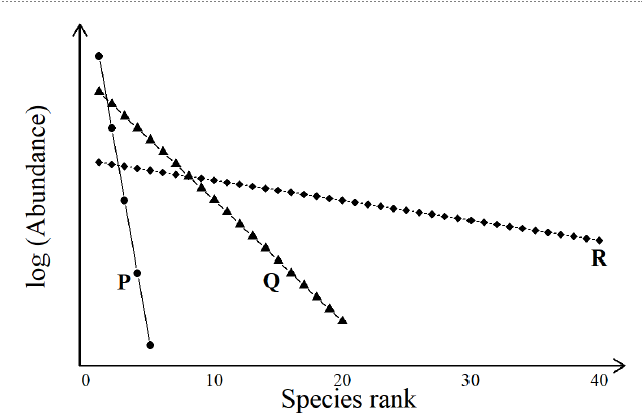
\includegraphics[width=0.8\columnwidth]{figs/Q-47.png}
    \label{Q.47}
\end{figure}
    \begin{enumerate}
        \item P $>$ Q $>$ R
        \item Q $>$ P $>$ R
        \item R $>$ Q $>$ P
        \item R $>$ P $>$ Q
    \end{enumerate}
\hfill{(GATE EY 2024)}

\item The graph shows bird species richness in a large contiguous forest patch and a small adjacent forest fragment, before and soon after the large contiguous forest patch was replaced by an oil palm plantation. Which one of the following options best explains the pattern shown?
\begin{figure}[!ht]
    \centering
    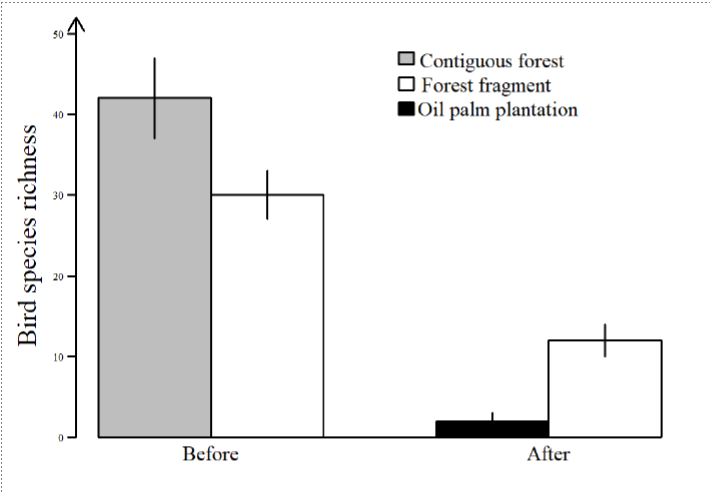
\includegraphics[width=0.8\columnwidth]{figs/Q-48.png}
    \caption{Question 48: Bird species richness before and after habitat conversion in a contiguous forest and a forest fragment.}
    \label{Q.48}
\end{figure}
    \begin{enumerate}
        \item The contiguous forest is a sink and the forest fragment is a source for bird species.
        \item The forest fragment has higher species richness than the contiguous forest.
        \item The bird community in the forest fragment is geographically closed.
        \item The contiguous forest was contributing to forest fragment species richness via dispersal.
    \end{enumerate}
\hfill{(GATE EY 2024)}

\item Honey bees are haplodiploid, which means that the relatedness is, on average, expected to be $0.35$ between
    \begin{enumerate}
        \item brother-brother pairs with the same parents.
        \item brother-sister pairs with the same parents.
        \item mated female-male pair.
        \item sister-sister pairs with the same parents.
    \end{enumerate}
\hfill{(GATE EY 2024)}

\item Match the mollusc taxa to their respective orders.
\begin{tabular}{ll}
\textbf{Mollusc taxa} & \textbf{Order} \\
I. Cone snails & P. Bivalve \\
II. Octopuses & Q. Gastropod \\
III. Giant clams & R. Cephalopod \\
IV. Squids & \\
\end{tabular}
    \begin{multicols}{2}
    \begin{enumerate}
        \item I-P; II-Q; III-R; IV-Q
        \item I-Q; II-R; III-P; IV-R
        \item I-P; II-R; III-P; IV-Q
        \item I-P; II-P; III-R; IV-Q
    \end{enumerate}
    \end{multicols}
\hfill{(GATE EY 2024)}

\item A terrestrial species P is found in both India and West Africa and nowhere else, while a marine species Q is found in the Arabian Sea and the Bay of Bengal. The two species have similar generation times. An ecologist builds haplotype networks based on DNA sequences from these species, where each circle represents one haplotype and each dash (-) represents a mutation. Which one of the following inferences is best supported by the haplotype networks shown?
\begin{figure}[!ht]
    \centering
    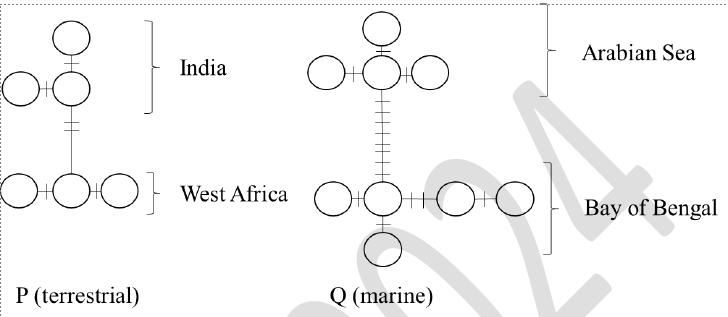
\includegraphics[width=0.3\columnwidth]{figs/Q-51.png}
    \caption{Question 51: Haplotype networks for a terrestrial species (P) and a marine species (Q).}
    \label{Q.51}
\end{figure}

    \begin{enumerate}
        \item P has high dispersal ability; Q has low dispersal ability.
        \item Q has high dispersal ability; P has low dispersal ability.
        \item P and Q have equal dispersal abilities.
        \item The genetic structure is not influenced by dispersal ability.
    \end{enumerate}
\hfill{(GATE EY 2024)}

\item Grey langurs found in the southern Western Ghats (SWG) and grey langurs in Sri Lanka (SL) look very similar. Nilgiri langurs (found in SWG) and purple faced langurs (found in SL) also look similar. If allopatry played a role in the early diversification of this group (at point $x$ in the tree), which one of the phylogenetic trees is most likely to be correct?
\begin{figure}[!ht]
    \centering
    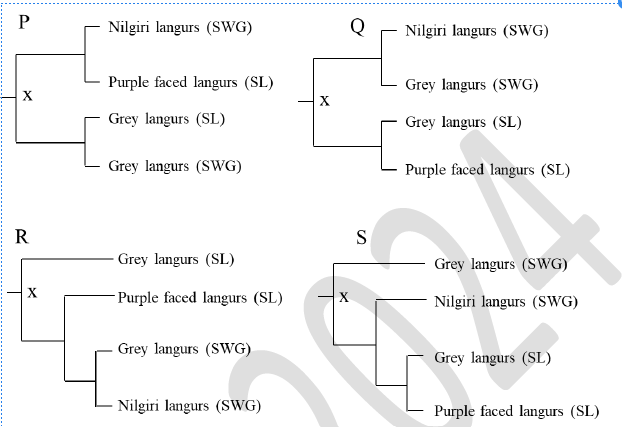
\includegraphics[width=0.8\columnwidth]{figs/Q-52.png}
    \caption{Question 52: Four possible phylogenetic trees (P, Q, R, S) for langur species from the southern Western Ghats (SWG) and Sri Lanka (SL).}
    \label{Q.52}
\end{figure}
    \begin{multicols}{2}
    \begin{enumerate}
        \item P
        \item Q
        \item R
        \item S
    \end{enumerate}
    \end{multicols}
\hfill{(GATE EY 2024)}

\item Two bird species, A and B, are found on a single mountainside. A is a low-elevation species, found between $500$ m and $1500$ m Above Sea Level (ASL), while B is a high-elevation species, found between $1000$ m and $2000$ m ASL. At $1250$ m ASL, species A and B have very different bill morphologies, but the bill morphology of species A at $500$ m is very similar to the bill morphology of species B at $2000$ m ASL. Which one or more of the following explain(s) the difference in bill morphology at $1250$ m ASL?
    \begin{multicols}{2}
    \begin{enumerate}
        \item Competitive exclusion
        \item Character displacement
        \item Convergent evolution
        \item Allopatric speciation
    \end{enumerate}
    \end{multicols}
\hfill{(GATE EY 2024)}

\item Which one or more of the following is/are greenhouse gas(es)?
    \begin{multicols}{2}
    \begin{enumerate}
        \item Methane
        \item Water vapour
        \item Sulphur dioxide
        \item Nitrous oxide
    \end{enumerate}
    \end{multicols}
\hfill{(GATE EY 2024)}

\item Males of the Indian robin in two populations sing songs of different lengths. Which one or more of the options given is/are an ultimate (not proximate) explanation(s) of the difference in song length between the two populations?
    \begin{enumerate}
        \item Females prefer to mate with males that sing longer songs in one population but not in the other.
        \item The two populations have different forms of the gene that determines song duration.
        \item The two populations differ in hormone levels that activate the start and end of singing behaviour.
        \item Differences between populations in food availability during development affect neural circuitry that is involved in song production.
    \end{enumerate}
\hfill{(GATE EY 2024)}

\item Female Anopheles mosquitoes bite humans to get blood. Researchers performed an experiment to study whether females use temperature or scent cues, or both, when locating human hosts. They presented female mosquitoes with membranes kept at different temperatures. Some membranes also had human scent applied to them. The response to each treatment was measured as the percentage of females that landed on the membrane ($50$ females for each treatment). The table shows the treatments and the corresponding responses.\\
\begin{tabular}{|p{6cm}|c|}
\hline
\textbf{Temperature and scent} & \textbf{Response} \\
\hline
Ambient air temperature ($25$ \degree C); with human scent & $90\%$ \\
\hline
Ambient air temperature ($25$ \degree C); without human scent & $0\%$ \\
\hline
Human body temperature ($37$ \degree C); with human scent & $90\%$ \\
\hline
Human body temperature ($37$ \degree C); without human scent & $90\%$ \\
\hline
\end{tabular}\\
Which one or more of the following inferences is/are supported by these results?
    \begin{enumerate}
        \item Human scent cues are necessary to locate human hosts.
        \item Human scent cues are sufficient to locate human hosts.
        \item Human body temperature cues are necessary to locate human hosts.
        \item Human body temperature cues are sufficient to locate human hosts.
    \end{enumerate}
\hfill{(GATE EY 2024)}

\item A phylogenetic tree for the evolution of two pigmentation traits in species of fish is shown for clades X, Y and Z. Genes A and/or B, if mutated, can cause dark pigmentation in the body. Which one or more of the following statements is/are correct?
\begin{figure}[!ht]
    \centering
    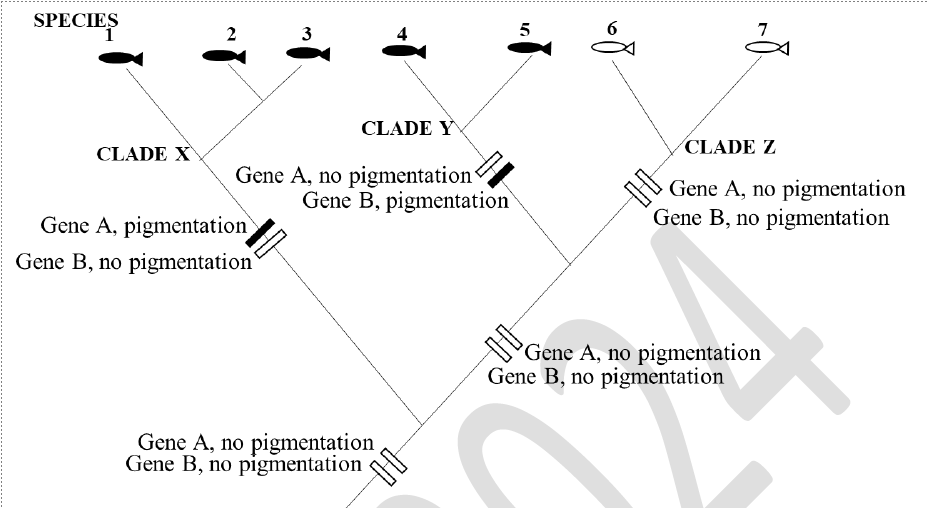
\includegraphics[width=0.8\columnwidth]{figs/Q-57.png}
    \caption{Question 57: Phylogenetic tree showing the evolution of pigmentation in three clades of fish.}
    \label{Q.57}
\end{figure}
    \begin{enumerate}
        \item The character state "pigmentation" is homologous in species $1$ and $3$.
        \item The character state "pigmentation" is homologous between species $1$ and $4$.
        \item The character state "pigmentation" is not homologous for species $6$ and $7$.
        \item The character state "pigmentation" is not homologous between species $2$ and $6$.
    \end{enumerate}
\hfill{(GATE EY 2024)}

\item In conservation biology, which one or more of the following is/are used to calculate the effective population size, $N_e$?
    \begin{enumerate}
        \item the population size required to avoid local extinction in the next $1000$ years.
        \item the carrying capacity of the environment.
        \item the sum of the sizes of all connected populations in a metapopulation.
        \item the number of breeding males and females.
    \end{enumerate}
\hfill{(GATE EY 2024)}

\item In the foodweb diagrams shown, R represents the primary producer, C1 and C2 represent intermediate consumers, and P represents the top predator. Which one or more of these diagrams show(s) intraguild predation?
\begin{figure}[!ht]
    \centering
    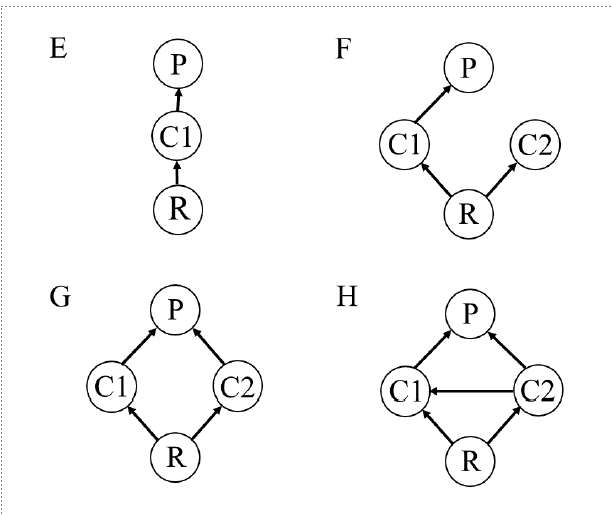
\includegraphics[width=0.3\columnwidth]{figs/Q-59.png}
    \caption{Question 59: Four food web diagrams (E, F, G, H) showing different trophic interactions.}
    \label{Q.59}
\end{figure}
    \begin{multicols}{2}
    \begin{enumerate}
        \item E
        \item F
        \item G
        \item H
    \end{enumerate}
    \end{multicols}
\hfill{(GATE EY 2024)}

\item You are a plant ecologist studying a plant in the genus \textit{Veronica}. You notice that, at open rocky sites, \textit{Veronica} grows as a creeper spreading low to the ground, whereas in grasslands, the stem stands upright. You collect seeds from multiple populations in each habitat type and grow them under uniform conditions in a greenhouse. You find that all the plants grown in the greenhouse have stems that stand upright. Which one or more of the following explanations best support(s) your observations?
    \begin{enumerate}
        \item The different morphologies in the natural habitat types are due to phenotypic plasticity.
        \item Inbreeding depression has led to the creeping form in the rocky sites.
        \item High gene flow between populations has restricted local adaptation in the two environments.
        \item The morphological differences between populations demonstrates that growth form is a polygenic trait.
    \end{enumerate}
\hfill{(GATE EY 2024)}

\item One hypothesis for why the tropics have far greater species richness than higher latitudes is that the tropics are relatively aseasonal. Low seasonality can encourage high species richness through which one or more of the following mechanisms?
    \begin{enumerate}
        \item Numerous resources are consistently available throughout the year, allowing different species to specialize on different resources, thereby minimizing competition and allowing co-existence.
        \item Low seasonality is associated with lower rates of predation, allowing large populations to thrive.
        \item Low seasonality is associated with more stable populations that are less vulnerable to demographic stochasticity and extinction.
        \item Low seasonality is associated with longer generation times, which enhances species richness.
    \end{enumerate}
\hfill{(GATE EY 2024)}

\item The figure illustrates the soil zinc tolerance of the grass species \textit{Anthoxanthum} along a transect from inside a mine to the middle of a pasture outside the mine. Which one or more of the following processes explain(s) the observed pattern of zinc tolerance in this grass species?
\begin{figure}[!ht]
    \centering
    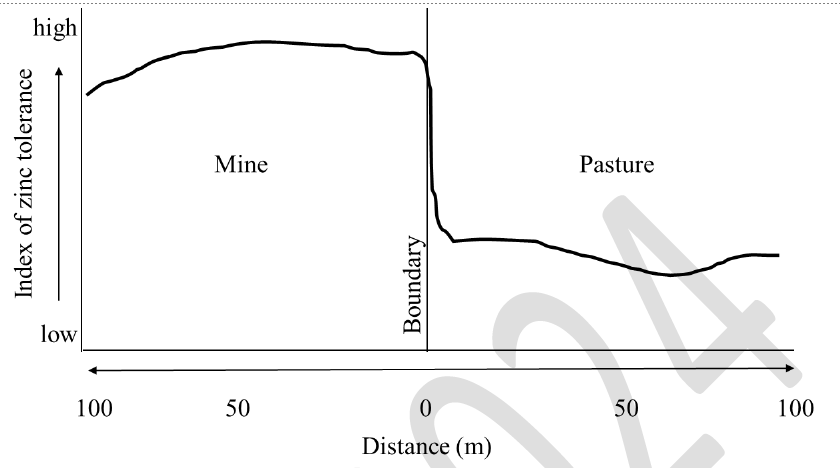
\includegraphics[width=0.8\columnwidth]{figs/Q-62.png}
    \caption{Question 62: Zinc tolerance of grass species along a transect from a mine to a pasture.}
    \label{Q.62}
\end{figure}
    \begin{multicols}{2}
    \begin{enumerate}
        \item Genetic drift
        \item Local adaptation
        \item Coevolution
        \item Introgression
    \end{enumerate}
    \end{multicols}
\hfill{(GATE EY 2024)}

\item In a forest, there are tigers, hare, and deer. On a given day, the probability of a tiger hunting a hare is $0.35$, a deer is $0.25$, and either a hare or a deer is $0.55$. The probability of a tiger hunting both a hare and a deer on a given day is \underline{\hspace{3cm}}. (Round off to two decimal places).
\hfill{(GATE EY 2024)}

\item Consider a discrete random variable $X$ that takes values from the set $S = \{0, 1, 2, 3\}$, being the number of individuals of a species within a habitat. Consider the probability distribution of $X$ with $Pr(X = 0) = 0.15$, $Pr(X = 1) = 0.25$ and $Pr(X = 3) = 0.5$, where $Pr$ denotes probability. The value of $Pr(X = 2)$ is \underline{\hspace{3cm}}. (Round off to two decimal places)
\hfill{(GATE EY 2024)}

\item There are nine species of \textit{Impatiens} (balsams) found in laterite plateaus of the northern Western Ghats, each with a distinct colour. If a plateau has exactly $6$ species, then the number of possible colour combinations in the plateau is \underline{\hspace{3cm}}. (Answer in integer)
\hfill{(GATE EY 2024)}

\end{enumerate}
\bigskip
\centering {\textbf{\large{END OF QUESTION PAPER}}}
\end{document}